%! Author = t
%! Date = 2025-02-05

\chapter{Physical Examination}\label{ch:ru_medical_examination}

\section{Intro}\label{sec:ru_}


The Chinese don't want you to come sick
(otherwise they'll have Vietnamese flashbacks),
so you need to collect some tests.
If you


\begin{note}
    Start preparing it immediately after
    you were nominated on exchange program by Innopolis.
    It takes a lot of time and efforts.
\end{note}



\section{Medical tests}\label{sec:ru_medical_tests}

To fill out this examination properly,
you must take the following tests:
\begin{itemize}
    \item Photofluorography
    \item Electrocardiography (ECG)
    \item Rh blood group system
    \item Human Immunodeficiency Viruses (HIV)
    \item Syphilis
    \item A certificate from a psychiatrist and addictionologist (narcologist)
    \item \textbf{Additionaly:} Vaccination list
\end{itemize}


Unfortunately, doctors in Innopolis hospital cannot fill out this form.
To fill out the form you should go to hospital in Kazan:

\textbf{Address:} Chuikova 54, terminal 2, 1st entrance,
2nd floor, office 2.8. Opening hours are 8:00-16:00.
\href{https://yandex.ru/maps/-/CHeHe8KC}{Yandex Maps}











\section{Can't finish examination on time}

On BIT website, you have to submit a completed examination before a deadline.
If you cannot complete it before,
you should receive mail in inbox on BIT website and fill the document Fig~\ref{fig:ru_med_state}.


\begin{figure}[htpb]
    \centering
    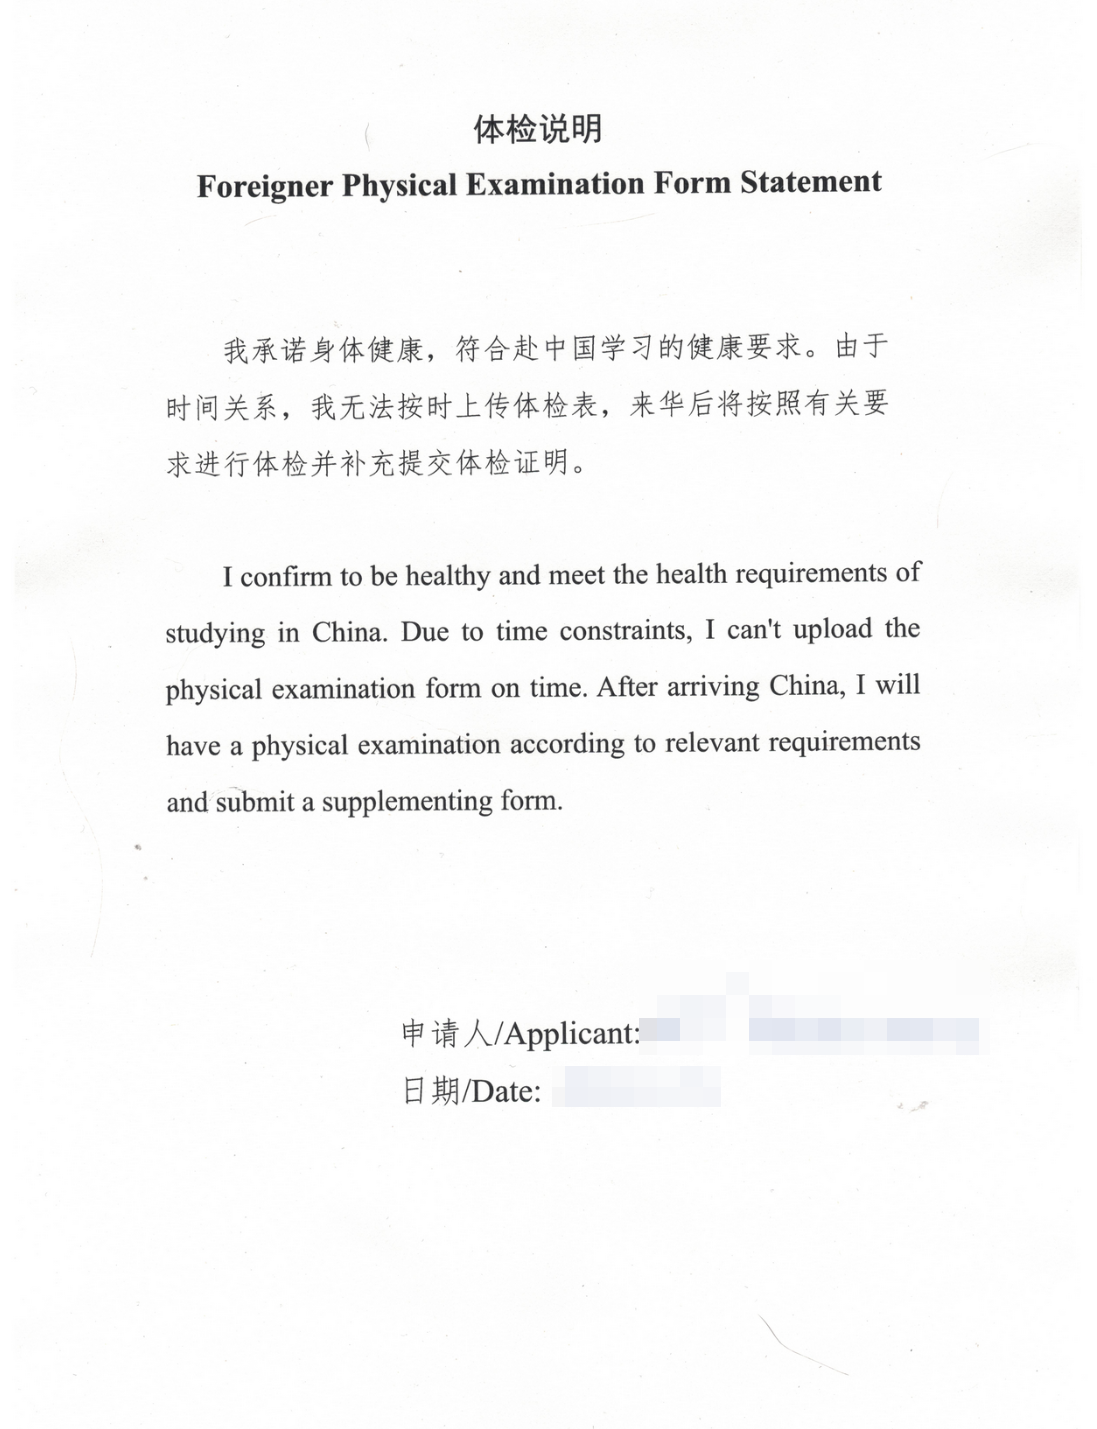
\includegraphics[width=0.8\textwidth]{russia/imgs/medical_statement}
    \caption{\centering Medical Examination Statement}
    \label{fig:ru_med_state}
\end{figure}
